\documentclass[12pt]{article}
% \usepackage[geometry]
% \geometry{a4paper}


\usepackage{mathtools}
\usepackage{tikz}
\usepackage{booktabs}
\usepackage{url}
\usepackage[utf8]{inputenc}

\usepackage[
    backend=biber,
    natbib=true,
    url=true,
    maxbibnames=99,
uniquename=init]{biblatex}

\def\layersep{2.5cm}
\def\outputlayer{5cm}

\bibliography{risk}
\begin{document}

\section{Introduction}
\label{sec:Introduction}

One of the recurring trends that is observable nowadays, is the active participation of single consumers in the financial markets~\cite{barasinska}. As such a clear development to support this in the banking sector has been created, where consumers are offered stocks, portfolios etc, which are tailored to their needs. This can be often lacking as individual preferences are not always accounted for, and most of the time standard questionnaires are used to classify customers in specific segments.

A metric which could actually be used with and would offer a little more certainty when creating suggestions for financial products tailored to the individual needs of a customer, is the willingness to take risk that each individual presents. As the risk of stocks and portfolio options can be calculated based on the expected returns, one could use this metric to asses which financial product would be appropriate for each individual.

Various researchers such as~\cite{individualRiskAttitude} have proposed a variety of determinants, and attributes which would express a certain level of risk-willingness or averseness in individuals. Although such metrics do not display causal relationships, but merely correlations, they could be used in conjunction with data-exploration algorithms such as machine-learning and deep-neural-networks to recognize common patterns between customers that display similar determinants.

The project described in this paper, was created with the purpose of allocating financial products of banks to their customers based on 4 preference questions. The questions should, in the end, provide a metric that would reflect the willingness to take risk for an individual customer. This metric would try to classify individuals in certain risk-classes which would then allow a bank-representative to make more concrete suggestions on the products offered to the customer.

Calculating financial risk though, is a very complicated manner. By recognizing that this problem is easy to solve although for an individual case, one might think that his is a problem of classifying individual in certain risk-category groups. The ability to provide classification from a variety of metrics, for a large number of data sets is a main feature exhibited by artificial neural networks. Thus, this paper will try to asses whether or not neural networks are a valid tool to solve such a problem.

For this reason, the project described in this paper will try to solve following problem:
\textit{Which metrics and how should those the metrics be evaluated using neural networks, in order to associate individual willingness to take risk with a specific risk class}

\section{Theoretical Background}
\label{sec:theoretical_background}

This section will provide a brief introduction into the main theoretical premises utilized in implementing this project. It is structured in the following way:

\begin{enumerate}
    \item The first subsection will provide a brief introduction into the definition of risk for financial products
    \item The second subsection will provide a brief introduction to neural networks and their functions
    \item Subsequently the application between the two will be explained
\end{enumerate}

After reading this Section, the reader will be able to grasp some of the technical aspects discussed in this paper, as well as some concepts related to machine learning and data sciences.

%TODO: Define the scope of financial risk discussed in this paper
% CITE: finRisk: https://is.muni.cz/el/1456/podzim2007/PMAEMA/Bouchaud_J.-P.__Potters_M._Theory_of_financial_risks.._from_statistical_physics_to_risk_management__CUP__2000_no_p.128-129_L_T_116s_.pdf
\subsection{Financial Risk}
\label{sub:financial_risk}
%TODO: Expand this section a tiny little bit
The measurement and control of risk is a major topic even today~\cite{finRisk}.~\cite{finRisk} states that financial risk is associated with the statistical uncertainty of the final outcome, and is measured by its volatility. Humans will indulge in financial risk at different levels, in order to arrive at financial gains. Some will indulge in highly risky affairs which yield higher rewards, while others will prefer less risk at the downside of smaller returns on their financial investment.

In the case of this paper, financial risk will be defined as the risk undertaken when a customer chooses to invests in a stock option, a portfolio or bond options with the ultimate goal of expanding his monetary gain. The financial risk undertaken therefore, is the loss of the investment in case of risk materialisation~\cite{finRisk}. The paper will not consider financial risk per se, rather it will consider itself with the risk category a customer is classified in based on his individual preferences, or in other words in the determinants chosen as part of the literary analysis.

\subsection{Neural Networks}
\label{sub:neural_networks}

Neural networks and deep learning are in essence machine learning algorithms, where deep learning is a more specific type of machine learning~\cite{deeplearningbook}. For the purpose of this paper, the definition presented below is derived from~\cite{deeplearningbook}. A machine learning algorithm foremost wants to learn something, anything that can be learned from a set of data, therefore a learning algorithm is employed.

\cite{mitchel97} defines the learning part of a learning algorithm as `A computer program is said to learn from experience \textit{E} with respect to some class of tasks \textit{T} and performance measure \textit{P}, if its performance at task in \textit{T}, as measured by \textit{P}, improves with experience \textit{E}.`. The task \textit{T}, is more accurately a task, that is difficult to solve with a fixed program, traditional program, and it is not to be confused with the process of learning, since the task itself is the problem that needs to be solved.


\subsubsection{The Task \textit{T}}
\label{subsub:task}
As iterated before, machine learning itself is a tool that allows one to solve a certain task, a problem, that is too difficult to be solved by a traditional fixed program designed by a human being.  Often people mistake the task itself with the process of learning, that is not the case. The task is the problem at hand, the learning process is the way in which the program can attain its ability, as for example a trainee who needs to learn from experience, to solve the task at hand~\cite{deeplearningbook}.

A machine learning task is usually described in terms how the machine learning system should process a certain example. The example itself is a collection of features which has been measured quantitatively from some source that the machine learning algorithm should process. The features themselves are described as $\textbf{x} \in R^n$ where each entry $x_i$ represents one feature out of all the recorded features.

The types of tasks and with it the type of networks that accompany it are briefly described in Section~\ref{subsub:task_types}. 

\subsubsection{Task Types}
\label{subsub:task_types}
The learning process is based on how a machine learning process will process an \textbf{example}, that is composed of a collection of \textbf{features}, where a vector $x \in R^n$ and each $x_i$ of the vector is just another feature of the example. An example of a feature are the values of the individual pixels in an image. Some of the more common tasks that can be solved by machine learning are as follows:

\begin{itemize}
    \item Classification: The task here is to specify in which category \textit{k} a certain input belongs to. These type of algorithms are used for example for classifying images to objects. A function $f(x)$is computed based on the data learned.
    \item Regression: The task here is to predict a numerical value given some input. The function $f(x)$ that is calculated is similar to the one of the classification algorithm with the exception that the output format differs. A simple example of this is the prediction of the claim amount an insured person will make, or the future price of securities.
    \item Transcription: The task in this instance, is to observe an unstructured representation of some kind of data, and try to transcribe it in textual form. A simple example of this is the transcription of a handwritten image to text.
    \item Machine translation: In this task the computer tries to translate one language to another, the most common application is the translation of two natural languages e.g. English to French. Here deep learning is quite important.
    \item Structured output: Any tasks, where the output is a vector, that contains important relationships between the different elements. An example is the transcription above, or parsing of natural languages in trees that describe grammatical structures.
    \item Anomaly detection: The program will flag data that is not conforming to the usually observed data as an anomaly. Usage is e.g. Credit card fraud, or in anti-virus software.
    \item Synthesis and sampling: The task is to generate new examples, based on the already existing data. This is interesting as for example the program might be tasked to create a movie script, or create large volumes of music.
    \item Imputation of missing values: The task is to be able to predict missing values in datasets
    \item Denoising: A corrupted example is given which was corrupted by an unknown process, and the program hast to predict a clean example through another clean example x
    \item Density estimation or probability mass function estimation:  Advanced use-case where the machine learns a probability density function
\end{itemize}
% Literature chosen based on what

\subsubsection{Performance Measure \textit{P}}
\label{subsub:performance_measure}

The performance measure evaluates, quantitatively how good the network performs for a specific task. As en example in the case of classification the measure would be the accuracy of the network in predicting correct results. Usually the performance is measured based on either the \textbf{accuracy}, that means the amount of correctly identified examples or the \textbf{error rate}, which designates the proportion of all the examples where the algorithm produces an incorrect output~\cite{deeplearningbook}.

To evaluate the performance measures after the reaching a satisfying error rate or accuracy, the performance is measured again based on a \textbf{test-set} of data that the network never saw before. These performance metrics though are not universal, and thus although it may seem straightforward it is not, since it has to often be decided how fine-grained, in what position and to which degree the error metric should be measured or penalized. All these considerations are part of the design phase of the network and are always depended on the type of task the network should perform~\cite{deeplearningbook}.

\subsubsection{The Experience, \textit{E}}
\label{subsub:the_experience}

Machine learning algorithms, as illustrated above can be split in either \textbf{supervised} or \textbf{unsupervised} learning algorithms. The experience discussed here is the is the \textbf{dataset} which is chosen as an input for the algorithm. 

In an \textbf{unsupervised} learning algorithm, the algorithm experiences the whole dataset and tries to extract useful properties out of it without requiring explicit labeling by a user, for example a denoising network, or a k-means algorithm. The algorithm itself basically always tries by viewing a set of examples $x$ to guess the probability distribution of y, or another interesting distribution which can be learned through the dataset. 

In a \textbf{supervised} learning algorithm, the algorithm experiences the dataset which is associated to a specific \textbf{label} or \textbf{target}. This is generally used as part of classification algorithms, such as when classifying plants based on the features of their iris. Generally speaking, a supervised learning algorithm tries to, by observing a dataset $x$ predict the probability of it being in $y$, so algorithmically guesses $p(y|x)$. 

The term supervised derives from the fact that the user of the network provides the network with a set of labels, such as an instructor in school where he provides the exercises and teaches the pupils what to do. In contrast, unsupervised training the algorithm tries to make sense from the data all by itself with no input from an instructor. The terms themselves are not really formally defined, and a clear distinction does not really exist, although this aspect is not in the scope of this paper.

Machine algorithms experience a certain dataset. The dataset can be usually thought of as a matrix where each row is one example of \textit{n} features. In supervised learning algorithms, the last column(s) of the matrix is usually reserved for for the \textbf{label y}. The label might often also not be a single number as an example the label could be a binary coded vector.
\subsubsection{Overfitting, underfitting and capacity}
\label{subsub:overfitting}

One of the most important and challenging aspects in machine learning is the concept of \textbf{over-} and \textbf{underfitting}. These two terms generally mean that due to outliers in the data the generated model either has a large gap between the training error and the test error, in the case of overfitting, or the training set cannot attain a low error value, as is the case when underfitting. 

These values can be controlled through an attribute called \textbf{capacity}. Capacity generally expresses a wide variety of functions, which will not be explained here, but one example would be to standardize the input data, in order to make it more homogeneous.

\subsubsection{Normalization, Standardization and One-hot-encodings}
\label{subsub:norm_stand_one_hot}

Normalization is not in any way connected with neural networks and machine learning as a concept, yet it is connected to the datasets the algorithms have to process. In statistics normalization can have a variety of meanings. The simplest case of normalization is the normalization of ratings, in which different rating measures are converted into a common scale. There is also the case of score normalization, in which different probability distributions are aligned onto a normal distribution.

In the case of this paper, normalization stands for the creation of shifted and scaled versions of statistics, where the intention is that these \textbf{normalized values} eliminate anomalies and big outliers in the dataset. Normalization can be used as a technique to avoid overfitting or underfitting data, and is expressed through following formula:

$x_new = (x - x_min)/(x_max - x_min)$

Standardization refers to  the conversion of data transforms the data in such a way that the data has zero mean and unit variance, and is described by following formula:

$x_new = (x - \mu) / \sigma$


One-hot-encoding stems from digital circuits, and in data-science it is employed when encoding categorical variables to values. Formally, when encoding categorical data one could use a values between \textit{1..n}, where \textit{n} amounts to the distinct elements in the categorical data. Usually though, it is not desired to have ordinal characteristics into a dataset that does not have any order such as male and female, where if male would be 1 and female 0 it would imply that female<male.

For this purpose, one-hot-encoding transforms these categorical data into binary encoded vectors, more formally, a single variable with \textit{n} observations and \textit{d} distinct values gets converted to a \textit{d} binary variable with \textit{n} observations each. Thus the example male female would be become (1,0) if the observation was male and (0,1) if the observation was female.

\subsubsection{Deep Neural Networks}
\label{subsub:deep_nets}

The main form of deep learning used in this paper is the so called deep feedforward network, also called multilayer perceptron, which also constitute the quintessential model for deep learning networks. The goal of a network is the approximation of some function f*. The models are called feedforward since data flows from the inputs towards the outputs, where no feedback connections exist. An alternate form of it would be a network which feeds the information it got from the computations back to itself, and those are called recurrent neural networks.

The reason these algorithms are called networks, is that they are a composition between functions which execute in a chain depending on the input. Backpropagation is used in order to feed the error described previously back into the networks weight. The name deep stems from the fact, that due to having more than 2 functions there is a certain depth to the network, in other words the intermediate hidden layers.

\section{Literature Review}
\label{sec:literature_review}

This section will be reviewing available literature that focuses on creating neural networks to asses risk in different settings. Some of the literature reviewed here do not directly apply to the case at hand, yet yield useful information in what kind of methodology that should be applied in order to create the implementation detailed further down in this paper.

\subsection{Determinants of Risk}
\label{sub:determinants_riks}
%TODO: Add another paper from our big collection!
\cite{dp4807.pdf} researches the question if it is possible at all possible to investigate individual risk attitudes using a survey. In the paper~\cite{dp4807.pdf}, try to asses the viability of using a hypothetical lottery, and risk self-assessment when measuring risk-attitudes of individuals. 

Their research is based on~\cite{individualRiskAttitudes}, and therefore their questions are modelled in a similar fashion. The researchers findings indicate that hypothetical lotteries and self-scaling questions are generally good indicators to measures someones risk attitude. The author though argue, that the heterogeneity of the results point out that it might be better to use more context specific questions based on the problem at hand. The results of this study influenced the decisions taken in Section~\ref{sec:methodology} while creating the survey for this paper.

A wide array of research exists in the social, financial and economical studies on the determinants of risk in individuals and in groupings. For the purpose of this paper, a number of those which address financial risk directly were chosen.~\cite{individualRiskAttitudes} states that it aimed to examine risk attitudes based on a large representative survey provided by SOEP\@. 

The study was then complemented by a smaller field study which examined the general willingness of an individual to take risk, based on the findings of the previous examination. The authors then expand their findings in order to correlate the general risk with more specific risk types such as smoking, financial risk and etc. In the findings the group concludes that indeed gender, age, height and the parental background correlate with risk attitude an individual displays. In addition to these determinants, choices such as investment in stocks and doing sports have been found to contribute to the willingness of an individual to take risk.~\cite{individualRiskAttitudes} used a financial lottery in order to verify these results in the field experiment, this approach will be used by this paper in Section~\ref{sec:methodology}.


\subsection{Financial risk with NNs}
\label{sub:financial_risk_nn}
%TODO: Finish this + add another paper
Finance is always a subject in statistics, as such a number of literature exists which employees neural networks in financial context.~\cite{instanbulStock} investigates the application of neural networks in the Istanbul stock market. 

Building on that research,~\cite{bitcoinNN} try to predict the evolution of bitcoin price. The authors opted for a simple neural network using Theano, and opting not to asses price-to-price predictions but rather, train the network depending on the trends following trend prices show: \textbf{up,margin and down}. Their implementation uses the predictions made by the network in order to decide on trading the bitcoins. In the case of up they always trade, in margin they do nothing and in down there is the option to short-sell. Their results are interesting, as the network correctly predicts, after a certain amount of time the trends in the price of bitcoin, and thus also trades successfully.

\cite{bitoinNN}, state in their results, that the predictions made by the network, seemed to good to be really true, since when compared to more advanced on-line learning algorithms, their smple network was outperforming the rest. The end result showed that the network itself did not really outperform and that the baseline profit was close to zero. The important takeaway from the research, is that due to the complexity of stock markets the code should always be reviewed for mistakes. For this paper the research here is relevant as it shows that alternative methods of stating a problem and structuring the data could yield important results.

\cite{04443437.pdf} discussed risk evaluation of project financing. Project financing is a way is a way to finance large scale public projects, and stems from PPPs, and the metric assessed by the authors is the overall risk posed by an entity when investing in such an endeavour. They use a total of 18 features, with one output value which describes the risk score computed by experts. The results are stated by the authors to be satisfactory, yet one of the problems with the training results, and in general was the low availability of input data. This research tho, shows that neural networks can be used in complex settings to asses risk, in which the features used are non-exhaustive.

It can be thus concluded that neural networks are actively being used in finance to account for a variety of subjects, often those subjects consider themselves with regression tasks, yet there are also instances in which classification problems are analyzed. Furthermore the application of neural networks has not been fully realized at present, with most classification systems using pure machine learning algorithms. The following section will investigate the usage of neural networks in various settings that relate with risk-classification.

\subsection{Various risk with NNs}
\label{sub:various_risk_nn}
%TODO: Add another paper

\cite{riskAssesmentInternalAuditing} starts of with introducing the subject of risk assessment, applied into internal auditing, where risk assessment usually is based on pattern recognition, due to the fact that an unexpected deviation is symptomatic of risk. It's application into internal auditing risk assessment can help auditors understand the underlying data that leads to an assessment. The example used, is that as an expert, only continuous exposure and experience can yield good results. If a network is exposed to the assessment of the experts, it will in the end figure out the combination of variables used by the expert in order to make is underlying assessment. Of interest is that the author compared the results taken by the neural network, and traditionally used statistical models. The author concluded that the neural network had made a positive impact and thus was more accurate than the statistical models.

\cite{14_1_3.pdf} tries to construct a neural network in order to asses the credit risk posed by clients at banks, when asking for a loan. The authors compared neural networks with the discriminant analysis performed usually by the banks. The results state that the neural networks do add value in terms of the correctly classified samples, by a margin of around 8\%. The authors state that although the network performed better, discriminant analysis should be used with neural networks, as discriminant analysis allows for an easier identification of the key variables that influence the end-result of the metric.

What can be seen in this section is that neural networks are a viable tool in predicting risk, and in general risk assessment of either sentiment, or concrete values. If the key features that actually influence the network are identified before usage of the network, the performance could be significantly better than traditional methods. Neural networks can also be seen as a valid complement to existing alternatives, where as pointed out by~\cite{14_1_3.pdf}, there are scenarios where a combination of techniques would yield better results.

\section{Methodology}
\label{sec:methodology}
\begin{figure}~\label{fig:net_design}
   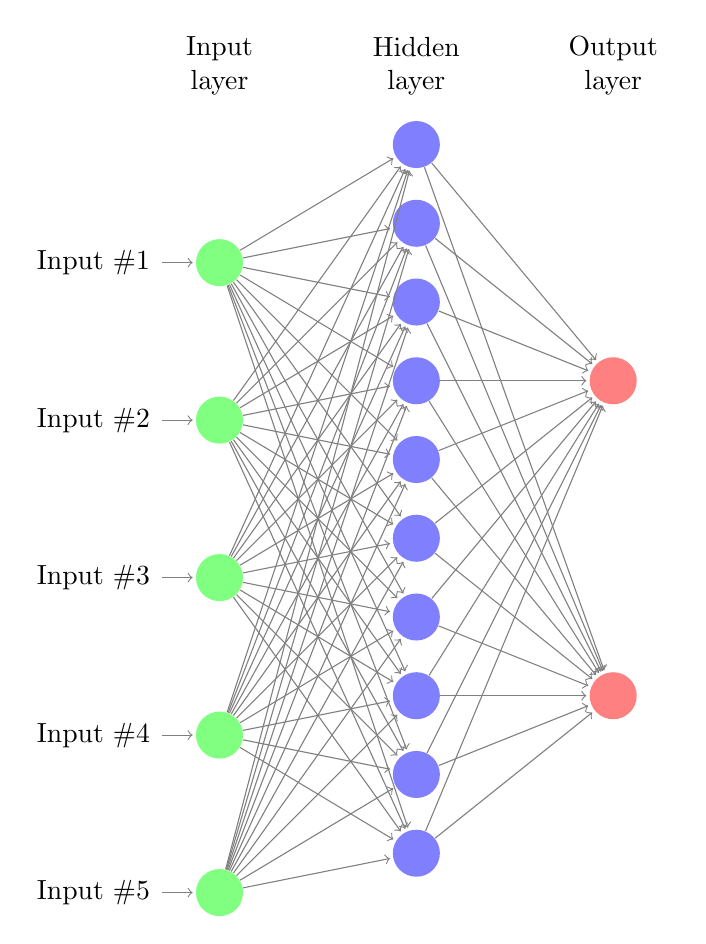
\begin{tikzpicture}[shorten >=1pt,->,draw=black!50, node distance=\layersep]
    \tikzstyle{every pin edge}=[<-,shorten <=1pt]
    \tikzstyle{neuron}=[circle,fill=black!25,minimum size=17pt,inner sep=0pt]
    \tikzstyle{input neuron}=[neuron, fill=green!50];
    \tikzstyle{output neuron}=[neuron, fill=red!50];
    \tikzstyle{hidden neuron}=[neuron, fill=blue!50];
    \tikzstyle{annot} = [text width=4em, text centered]

    % Draw the input layer nodes
    \foreach \name / \y in {1,...,5}
    % This is the same as writing \foreach \name / \y in {1/1,2/2,3/3,4/4}
        \node[input neuron, pin=left:Input \#\y] (I-\name) at (0,-\y*2 cm) {};

    % Draw the hidden layer nodes
    \foreach \name / \y in {1,...,10}
        \path[yshift=0.5cm]
            node[hidden neuron] (H-\name) at (\layersep,-\y cm) {};

    % Draw the output layer node
	\foreach \name / \y in {1,...,2}
		\path[yshift=0.5cm]
			node[output neuron] (O-\name) at (\outputlayer,-\y*4 cm) {};;

    % Connect every node in the input layer with every node in the
    % hidden layer.
    \foreach \source in {1,...,5}
        \foreach \dest in {1,...,10}
            \path (I-\source) edge (H-\dest);

    % Connect every node in the hidden layer with the output layer
    \foreach \source in {1,...,10}
		\foreach \dest in {1,...,2}
        	\path (H-\source) edge (O-\dest);

    % Annotate the layers
    \node[annot,above of=H-1, node distance=1cm] (hl) {Hidden layer};
    \node[annot,left of=hl] {Input layer};
    \node[annot,right of=hl] {Output layer};
\end{tikzpicture} 
\caption{Perceptron Network Architecture} 
\end{figure}

As detailed in the relevant literature, the methodology which is appropriate neural network design for the problem detailed in the introduction, is that of a multi-layered perceptron, using logistical regression at its output layer. As detailed in Section~\ref{sub:neural_networks} these types of networks are appropriate for classification tasks, and since the task as hand is to sort people based on their risk-attitude this designates it as a classification problem, as classifying people based on their political beliefs would be. The design of the network to be implemented can be visualised in Figure~\ref{fig:net_design}. 

To determine the relevant setup a questionnaire was developed based on the literature reviewed in~\ref{sub:determinants_risk}. The questionnaire is included as part of this paper in the appendix. The first assumption that is going to be tested is if the network can asses through the first three questions posed, the outcome of the fourth question. If the fourth question can be guessed correctly then we could equally assume that with the inclusion of the fourth question as an input the outcome will be even more correct. 

The purpose of the fourth question is to classify the persons answering the questionnaire into three distinct classes. One who is risk-averse, one who is of medium risk-aversity/propensity and a class who is more risk-prone than the other ones. The purpose of this, as detailed in Section\ref{sec:Introduction} is to be able to determine the appropriate investment packages that should be recommended to a client of a bank.
%TODO: Theano Graph
In order to be able to handle a small dataset, cross-validation is to be employed. At the network proceeds to plot the cross entropy validation of the validation and test loss with respect to the epochs run, which were detailed in Section~\ref{sub:neural_networks}. The prediction function will then be tested again on a small subset of the test set in order to be able to also visualize its accuracy. These graphs can be visualized in~\ref{fig:sampleGraph}

At the end, the results will be compared with the output of a Support Vector Machine, which can also be used in classification problems, and has been proven by research to be more suitable for certain classification problems. The neural network used here is using logistic regression, since the classification can be also seen as a recessionary problem, although the output values y are not continuous.
\subsection{The Questionnaire}

The questionnaire was created with the help of Questback Software. The questionnaire consist of 5 questions. The questions are structured in the following manner:
\begin{itemize}
    \item Start-page:
        \begin{itemize}
            \item Gender: Male or Female
            \item Age: Free numerical age entry
        \end{itemize}
    \item Risk-Questions:
        \begin{itemize}
            \item Lottery Question: How much would you be willing to pay for a lottery, consisting out of 100 tickets, where each ticket costs 15 Euro, and has a payout of 1000 Euros
                This question is a modified questions of the one found in~\cite{10.1.1.558.6537.pdf}. It is a modified lottery, in which the more tickets a user buys the higher his risk attitude is, since the reservation price would be higher.
            \item Risk self-assessment: This question is on the scale from 1-to-10 where the questioned party can choose the level of risk-engagement himself has as perceived by him
        \end{itemize}
    \item Modified Lottery: You have 10000 Euros to be allocated in following ways:
        \begin{enumerate}
            \item Risk-free Asset, with a compound interest of 3\% that pays out in 3 years
            \item A stock option, in which risk is around 50\% whereas if the stock is good the payout will be with a compound interest of 8.8\% over 3 years (13000 in total) and if it goes bad the payout will be 8000 
            \item A risky portfolio, in which compound interest is \~20\%(~150000 payout) in 3 years where if the investment goes bad, the totality of the money is lost. Risk is \~70\%
            \item No Investment
        \end{enumerate}
        This question aims to evaluate the risk propensity the questioned person has towards an asset, given his willingness to risk money in order to generate profits.
\end{itemize}

The questionnaire  is based on the determinants extracted from the literary review done in Section~\ref{sub:determinants_riks}. The questions are slightly more modified to suit the needs of this research, and in addition are kept in a low scope as a bigger questionnaire would require more specialized knowledge.

The questionnaire was to be distributed between the 15.09 and 15.10 of 2016,  but due to the limited time and participation, was only partly distributed. As such the data gathered by the questionnaire is deemed to not be sufficient enough to warrant an analysis by a neural network.

\subsection{Experiment}

Due to lack of data from the questionnaire, another dataset had to be chosen which would be similar to the input that was to be generated by the questionnaire. For this purpose the machine learning database of UCI, was used. Many datasets were found to be similar, but not quite, to the application domain of the questionnaire. For the experiment following datasets were chosen:

\begin{itemize}
    \item Bank: This dataset was created by~\cite{bank.names}, and relates to a direct marketing campaign of a Portuguese banking institution. The label is the correct prediction when a client will subscribe to a bank term deposit, and consists of 45211 entries which encompass 16 features. An overview of the dataset is included in~\ref{fig:bank_set_description}
    \item Adult: This dataset is provided by~\cite{adult.names}. It encompasses 48842 entries which encompasses 15 features, and the prediction label is whether an adult earns more or less than 50k.
\end{itemize}

The experiment has following setup:
\begin{itemize}
    \item First train the network, and create models one for a feed forward neural network, using indexed datasets
    \item The training itself should test a variety of activation functions
    \item After training the neural network, create one-hot-encoded labels and test them again to view the differences, and determine which is better suited for the task at hand
    \item Finally compare the resulting neural network models with an SVM\@.
\end{itemize}

The end result, will be to asses the viability of such networks in non-homogeneous financial data, and their ability to determine customer feedback in a `risky' proposition.

\section{Implementation Details}
\label{sec:implementation_details}

In the following the implementation of the network will be briefly explained. The core components implemented using Theano will be explained in addition to the command line options that can be used to manage the implemented network.

\subsection{Network Design}
\label{sub:network_design}

The chosen language for the implementation is python. This is due to the wide use in neural networks, and in general data-science which is enjoyed by python. As we needed a network with adequate performance the Theano~\cite{theanoTutorial} framework was chosen in order to implement the different neural network functionalities. Theano also did provide most of the activation functions by itself, the only exception of this was the Gaussian activation function which was to be implemented by hand. 

Although implemented, the function did not work as expected and thus was not considered as part of the experiment. Since Theano is quite a complex framework the implementation chosen for the task at hand was a simple feed-forward network with backpropagation as depicted in Figure~\ref{fig:sampleNetwork}

Theano computes its functions and generates internal graphs, the graph for the neural network created for this paper is depicted in Figure~\ref{fig:theanoGraph}. Due to the way Theano works it is also quite hard to debug it, or understand the internal workings in such a short time period. For this reason, the program employees the Keras framework~\cite{keras} to solve problems such as employing batch gradient descent on one-hot-encoded labels. Keras was chosen as it is based on Tensorflow, another popular library like Theano, and can also use Theano as its backend, in addition the standard implementation is also able to handle one-hot-encoded labels.

\subsection{Input Pre-processing}
\label{sub:splitfunc}

Since there can be different types of data, an additional splitting algorithm is employed which will pre-process the dataset in question, in order to first one-hot-encode the categorical data, then apply normalization where appropriate and later on split the dataset into the appropriate training, validation and testing sets. One-hot-encoding is needed in order to obtain sane values for binary and categorical datasets as explained in Section~\ref{subsub:norm_stand_one_hot}. To accomplish this task the \textbf{pandas} framework is used in order to do the one-hot-encoding. 

Following this, pandas is again employed in order to normalize all the columns of the dataset, which contain the feature set. Normalization is needed in order to restrict the data between the values of minimum and maximum values that it can acquire and is employed in statistics in order to reduce outliers as detailed in Section~\ref{subsub:norm_stand_one_hot}. 

In our case the normalization is crucial in order to also control overfitting and underfitting of the weights and the bias. While standardization is always a normalization, normalization itself is not a standardization. The effect of the normalization on the trained model can be seen in Section~\ref{sec:results}.

\subsection{Program Usage}
\label{sub:program}

The main scale of the program is located in the file \textit{run.py}. The file can be called using \textit{python run.py} with following arguments:
\begin{itemize}
    \item -d or --demo: runs the demo function on the MNIST dataset
    \item -pd or --prediction-demo: runs the MNIST prediction demo 
    \item -j or --json: expects a JSON as input with the task to solve
    \item -s or --split: expects a CSV as input and then splits the file into appropriate training, validation and test set
    \item -o or --no-ordinal: in combination with -s, no-ordinal produces a one-hot-encoded label
    \item -n or --no-normalize: in combination with -s, no-normalize produces non-normalized data-sets
    \item -v or --version: displays the program version
\end{itemize}

% \url{http://yann.lecun.com/exdb/mnist/}

\subsubsection{The Demo}
\label{subsub:demo}
The Demo consist of predicting the MNIST Dataset provided from~\cite{MNISTSite}. It is used as part of the Tutorial in~\cite{deepLearning.org}, and thus is used to demonstrate and test the custom build network. 

The Demo loads the MNIST Dataset from a python pickle file and then runs the network. The prediction part of the demo is run automatically when the prefix \emph{-d} is used. Alternatively if someone wants to just test how the predictor works, he can just activate the \emph{-pd} option.

The algorithm should run in a similar fashion as explained by~\cite{theanoTutorial}. The program is modelled after the algorithms introduced there albeit with a lot of modified parts in order to account for the differences of the datasets.

\subsubsection{JSON-Tasks}
\label{subsub:json}

The configuration of the tasks that should run in the neural network is given using a json file which is structured in the following way:
\begin{verbatim}
    {
        "tasks":[
                {
                    //Here Task Content    
                },...
                {
                    //Here Task Content 
                }
        
        ]
    }
\end{verbatim}

There are 2 key settings in the JSON file, which determine the overall contents of a single task entry. The variable in question is also called setting, and can be set to either train or predict. A Task then has following structure depending on the setting:

\begin{itemize}
    \item If the setting is set to \textbf{train} then following settings apply:
    \begin{itemize}
        \item \emph{learning\_rate}: This specifies the learning rate of the network.
        \item \emph{L1\_reg}: Used for rate regularization. 
        \item \emph{L2\_reg}: Same as above.
        \item \emph{training\_epochs}: How many epochs should the network maximally train
        \item \emph{datasets}: A collection of datasets that the network should calculate
        \item \emph{n\_outs}: The amount of output nodes present in the network
        \item \emph{batch\_size}: How many batches should be used in each epoch
        \item \emph{n\_hidden}: Specifies the size of the hidden layers. If given as list will produce multiple hidden layers
        \item \emph{logfile}: A file which would log the output of the training
        \item \emph{activation}: The activation function to be used, currently supports: \textit{tanh(x),relu(x),gausian(x),sigmoid(x),hard\_sigmoid(x)}
        \item \emph{delimiter}: Specifies the delimiter to be used in the logfile and the delimiter which is present in the dataset input file
    \end{itemize}
    \item If the setting is set to \textbf{predict}:
        \begin{itemize}
            \item \emph{best\_model}: The pre-calculated model for the neural network
            \item \emph{datasets}: The dataset which was used in the training 
            \item \emph{n\_outs}: Same as above
            \item \emph{n\_hidden}: Same as above
            \item \emph{result\_file}: File to store prediction results
            \item \emph{delimiter}: Same as above
            \item \emph{activation}: Be sure to use the same activation function used to generate the model
        \end{itemize}
\end{itemize}

In addition the program can also be run using the GPU, though currently due to the lack of a testable computer this function is still not implemented, as Theano only fully supports NVIDIA-CUDA\@. The necessary  information to craft the prediction task runs can be extracted from the logfile that was created while training the network.

\subsubsection{The Dataset}
\label{subsub:dataset}

The dataset should be provided as a single CSV\@. Then the user has to split the dataset into a training set, a validation set and a testing set. To simplify this process for the user, the neural network implements the -s argument which calls the CSV splitter, discussed as part of Section~\ref{sub:splitfunc}. 

The splitter takes the file and splits it into an 80/20 training/test file, it then proceeds to apply a similar 80/20 split to the training file in order to provide a fair validation set. In the JSON file which serves as an input to the neural network, the user has to mainly write the name of the original CSV file, the program takes care of it itself.

\subsubsection{The Splitter}
\label{subsub:splitter}

The splitting sub function is located under \emph{split.py}. It receives as input the totality of the dataset, and the proceeds to produce training, validation and testing sets for the dataset in question. In order to produce this, it uses and 80-to-20 split for the training and testing set, and subsequently again an 80-to-20 split between the acquired training set and subsequent validation set.

The data is then standardized using one-hot-encoding, which basically splits categorical data. The data is then normalized, using the average mean, of the rows. The target labels are currently not normalized as in Theano, Y also acts as the index calculator, and thus a transformation in floats would not serve any purpose.

\subsubsection{Tackling Multiclass Problems}
\label{subsub:multiclass_problem}

When trying to solve a multiclass problem, you will often stumble upon the alternative of either specifying classes as numeric entities, or the better alternative to use a one-hot-encoding on the Labels, which subsequently removes the ordinal bias a numerical representation of the classes would have. 

As such, and since one might want to observe the difference in performance between one-hot-encoded variables and indexed classification, an alternative was to be implemented that handles one-hot-encoded target labels. As explained previously one-hot-encoded data presents the target values as pairs, depending on the class that they represent, also called binary encoding. An example of such an encoding is located in Table~\ref{tab:oneHot}.

In order to simplify the implementation, such multiclass problems are handled by \emph{Keras} framework, as this was the most optimal way to implement it. For this, the output dimension is calculated and thus assessed if an index labeled dataset is used, or a one-hot-encoding variant, in a case of a one-hot-encoded dataset, the Keras implementation is called. 

The implementation itself is a more simplistic as the one implemented with Theano, as it serves a specific purpose, namely to compare the results of the logistic regression network with an alternative implementation, and also to display the difference one-hot-encoding plays for the particular type of datasets available.

\subsubsection{The Prediction Function}
\label{subsub:prediction}

The prediction function works in the following way:
\begin{enumerate}
    \item Load the specified datafile into the shared memory
    \item Load the trained model and construct the network
    \item Subsequently (for the test runs) print the expected results
    \item Excecute the prediction function
    \item Print the results on the screen and in addition to a predition file
\end{enumerate}

The prediction function is not tied to the training function in any way, and thus other models trained by Theano for similar networks can be loaded and used.

\section{Results}
\label{sec:results}

\begin{table}[h]
   \centering
   \caption{JSON-Table}
   \label{tab:JSON}
   \begin{tabular}{lcccccccc}\toprule
        Dataset & Learning Rate & L1 Reg & L2 Reg & Epochs & In & Hidden & Out & Batch-Size \\
        \midrule
        bank\_normalize & 0.0001 & 0.00 & 0.0001 & 1000 & 51 & 51 & 2 & 10 \\
        bank & 0.0001 & 0.00 & 0.0001 & 1000 & 51 & 51 & 2 & 10 \\
        adult\_normalized & 0.0001 & 0.00 & 0.0001 & 1000 & 51 & 51 & 2 & 10 \\
        adult & 0.0001 & 0.00 & 0.0001 & 1000 & 51 & 51 & 2 & 10 \\ 
        \bottomrule
   \end{tabular}
\end{table}
The network was tested with different configurations. In Figure~\ref{tab:JSON}, represents the end configuration that yielded the maximum results for most activation functions. In Table~\ref{tab:interResults} the intermediate results of some network configuration can be visualised. In Figure~\ref{fig:graphs} the individual progressions of the gradient descent can be visualized.

\begin{table}[h]
    \centering
    \caption{Intermidiate Results}
    \label{tab:label}
    \begin{tabular}{c}
    
    \end{tabular}
\end{table}

The bank\_2 dataset is a non normalized on in order to show to the impact between a normalized and a non normalized dataset. The bank dataset was extracted from UCI Database, as it was determined to be the set better suited to the application scenario of the network. The network is not quite accurate as it has a loss of 10\%, although it is enough to start making some predictions. An optimal way to increase the networks accuracy is to have a larger dataset, in order to be able to increase the training data for the network. 

The best activation function was determined to be \emph{tanh}, which produced the best results for the validation and the test set, as can be seen in Table~\ref{tab:taskRuns}. The differences between the activation functions are minimal although one can observe that the end results of the testing set that there is quite a significant differences between validation and testing. This can actually be attributed to the size of the testing set itself.A larger dataset would likely produce more accurate results, and also have given a lower error when validating the new model with the testing set.

\begin{table}[h]
    \centering
    \caption{Results SVM and NeuralNet Task Runs}
    \label{tab:taskRuns}
    \begin{tabular}{c}
    
    \end{tabular}
\end{table}

HERE COMES THE SVM
%TODO: Implement an SVN?
%TODO: Using an SVM these results. Then type here how it compares to the neural network

\section{Future Work}
\label{sec:future_work}

As can be seen, although not accurate the neural networks can actually be used to predict the choices a person would make when faced with risk-based decision in a financial situation. It is also possible that with even more data, and a lot more features for the dataset, the prediction could have been more accurate than the current program output. Further work in this direction would entail the creation of a more elaborate questionnaire and a higher population sampling.

Many improvements could also be added to the algorithm generating the neural network, for example an option to add a lot more hidden layers with variable node count. In addition, other output layers could also be implemented that do not directly implement logistical regression but rather other methods of inferring the results of the network, such as an unsupervised recurrent neural network. 

Fortunately such frameworks do exists, for example  the already employed Keras Framework~\cite{keras}, or the Lasagne Framework~\cite{lasagne}, or which offer a higher level of abstraction and thus an easier way to construct neural-networks. In addition, other methods for gradient descent could be considered that are more optimal than batch-gradient descent, or better weight initialization.

All in all the program has served the purpose of showing the concept of neural networks used in determining deciscions undertaken by person when faced with a decision making process, may this be an answer to the proposal of his bank for a product offered by it, or in order to asses the financial liquidity of a person to help infering a decision.

\printbibliography{}
\end{document}
